\chapter{Conceptos sobre Rankings}
En este capítulo explicaremos todos los conceptos y herramientas necesarios relativos a rankings. Comenzaremos diferenciando los dos conceptos alrededor de los cuales girará todo el capítulo: ranking y rating. Una vez explicado qué es un ranking y qué un rating, veremos cuatro métodos para poder generarlos a partir de diferentes estadísticas: el de Massey, el de Colley, el de Keener y el de Ataque-Defensa. Una vez que sepamos cómo crear varios rankings a partir de los métodos antes vistos, podemos combinarlos para generar super-rankings más robustos. Es lo que llamaremos agregación de rankings y veremos tres métodos distintos para hacerlo. En la cuarta parte del capítulo estudiaremos distintas herramientas para realizar comparaciones entre rankings y ver el grado de concordancia entre ellos. Para terminar el capítulo haremos un estudio de cómo los ítems van intercambiando sus posiciones en los rankings, introduciendo el término competitividad con su correspondiente representación en los grafos de competitividad. 

\section{Rankings vs Ratings}
A menudo se utilizan ambos términos de forma indistinta, sin embargo, hay claras diferencias entre ellos, \cite{cap1}

\subsection{Rankings}
\begin{defi} 
	Un \textbf{ranking} de tamaño n es una permutación de enteros desde 1 hasta n, es decir, se trata de una biyección $r: \xi \rightarrow \xi$ donde $\xi = \{1,...,n\}$ es el conjunto de elementos a ordenar.
\end{defi}
A partir de ahora los veremos representados como un vector columna en el que cada posición del vector (que coincidirá con alguno de los elementos que queremos ordenar) se corresponderá con un número entero que indica la posición que ocupa dicho elemento en el ranking. 
 
\newpage 
 
\begin{ejem} \label{ejem1}
A continuación se muestra el ranking de la clasificación de la liga ACB del año 2014/2015 al finalizar la fase regular:
\end{ejem}
	
\[
\begin{array}{ccc}
\begin{array}{c}
\text{Baloncesto Sevilla}\\
\text{CAI Zaragoza} \\
\text{Dominion Bilbao Basket} \\
\text{FC Barcelona} \\
\text{FIATC Joventut} \\
\text{Gipuzkoa Basket} \\
\text{Herbalife Gran Canaria} \\
\text{Iberostar Tenerife} \\
\text{La Bruixa d'Or Manresa} \\
\text{Laboral Kutxa Baskonia} \\
\text{Montakit Fuenlabrada} \\
\text{MoraBanc Andorra} \\
\text{Movistar Estudiantes} \\
\text{Real Madrid} \\
\text{Río Natura Monbús Obradoiro} \\
\text{UCAM Murcia} \\
\text{Unicaja Málaga} \\
\text{Valencia Basket Club}

\end{array} & \left(\begin{array}{c}
15\\
9\\
4\\
2\\
7\\
17\\
8\\
11\\
16\\
6\\
18\\
14\\
13\\
1\\
12\\
10\\
3\\
5
\end{array} \right)
\end{array}  
\]
\qed
\ \\

Si $e$ es un elemento del conjunto a ordenar, $r(e)$ es la posición que ocupa el elemento $e$ en el ranking $r$, en el ejemplo \ref{ejem1}, $r(\text{Baloncesto Sevilla}) = 15$.

\subsection{Ratings}
\begin{defi} 
	Un \textbf{rating} es una lista de puntuaciones numéricas, una por cada elemento, es decir, $\tilde{r}: \xi \rightarrow \mathbb{R}$ donde $\xi = \{1,...,n\}$ es el conjunto de todos los elementos.
\end{defi}
Se representan de forma análoga a los rankings, cada elemento se corresponderá con una puntuación (partidos ganados, perdidos y empatados, puntos a favor y en contra, porcentajes,...).\\

Ordenando un rating, siempre se obtiene un ranking, pero no a la inversa. Por ejemplo, el ranking del ejemplo \ref{ejem1} es el obtenido a partir del rating del ejemplo \ref{ejem2}.

\newpage  
 
\begin{ejem} \label{ejem2}
 A continuación se muestra el rating de partidos ganados de la ACB del año 2014/2015:
\end{ejem}
	
	\[\begin{array}{ccc}
	\begin{array}{c}
	\text{Baloncesto Sevilla}\\
	\text{CAI Zaragoza} \\
	\text{Dominion Bilbao Basket} \\
	\text{FC Barcelona} \\
	\text{FIATC Joventut} \\
	\text{Gipuzkoa Basket} \\
	\text{Herbalife Gran Canaria} \\
	\text{Iberostar Tenerife} \\
	\text{La Bruixa d'Or Manresa} \\
	\text{Laboral Kutxa Baskonia} \\
	\text{Montakit Fuenlabrada} \\
	\text{MoraBanc Andorra} \\
	\text{Movistar Estudiantes} \\
	\text{Real Madrid} \\
	\text{Río Natura Monbús Obradoiro} \\
	\text{UCAM Murcia} \\
	\text{Unicaja Málaga} \\
	\text{Valencia Basket Club}
	\end{array} & \left(\begin{array}{c}
	12\\
	18\\
	20\\
	25\\
	19\\
	10\\
	18\\
	16\\
	11\\
	19\\
	8\\
	12\\
	14\\
	27\\
	15\\
	17\\
	25\\
	20
	\end{array} \right)
	\end{array}\]
\qed

\begin{ejem} A continuación se muestra el rating de diferencia de puntos de la ACB del año 2014/2015 con su correspondiente ranking tras ordenarlos:
\end{ejem}	
	$$\begin{array}{ccc}
	\begin{array}{c}
	\text{Baloncesto Sevilla}\\
	\text{CAI Zaragoza} \\
	\text{Dominion Bilbao Basket} \\
	\text{FC Barcelona} \\
	\text{FIATC Joventut} \\
	\text{Gipuzkoa Basket} \\
	\text{Herbalife Gran Canaria} \\
	\text{Iberostar Tenerife} \\
	\text{La Bruixa d'Or Manresa} \\
	\text{Laboral Kutxa Baskonia} \\
	\text{Montakit Fuenlabrada} \\
	\text{MoraBanc Andorra} \\
	\text{Movistar Estudiantes} \\
	\text{Real Madrid} \\
	\text{Río Natura Monbús Obradoiro} \\
	\text{UCAM Murcia} \\
	\text{Unicaja Málaga} \\
	\text{Valencia Basket Club}	
	\end{array} & \left(\begin{array}{c}
	-211\\
	-66\\
	+45\\
	+351\\
	+28\\
	-239\\
	+2\\
	+32\\
	-216\\
	+165\\
	-185\\
	-66\\
	-106\\
	+263\\
	-68\\
	-39\\
	+154\\
	+142
	\end{array} \right) & \left(\begin{array}{c}
	16\\
	11\\
	6\\
	1\\
	8\\
	18\\
	9\\
	7\\
	17\\
	3\\
	15\\
	11\\
	14\\
	2\\
	13\\
	10\\
	4\\
	5
	\end{array} \right) 
	\end{array}$$
\qed

\newpage

\section{Métodos para crear rankings}
En esta sección vamos a ver distintas maneras de obtener ratings usando algunas de las estadísticas disponibles (victorias, derrotas, puntuaciones, \dots) y posteriormente ordenarlos para crear nuevos rankings. Concretamente veremos cuatro de ellas: el método de Massey \cite{cap2}, el método de Colley \cite{cap3}, el método de Keener \cite{cap4} y el método de ataque-defensa \cite{cap7}. Podemos encontrar otros métodos en \cite{otros_met}.

\subsection{Método de Massey}
Este método fue propuesto por Kenneth Massey en 1997 y está basado en la teoría matemática de mínimos cuadrados.\\

La idea principal se puede resumir en la siguiente ecuación: 
\begin{equation}
	r_{i}-r_{j} = y_{k}
\end{equation}
donde $y_{k}$ es el margen de victoria para el enfrentamiento entre los equipos $i$ y $j$, y $r_{i}$ y $r_{j}$ son los ratings del equipo $i$ y $j$ respectivamente.\\
\\
O lo que es lo mismo, la diferencia entre los ratings del equipo $i$ y $j$ nos permite predecir cual será el margen de victoria en el enfrentamiento entre los equipos $i$ y $j$.\\

Para obtener el vector de ratings $r$ por Massey se tiene que resolver el siguiente sistema de ecuaciones:
\begin{equation}
	Mr = p
\end{equation}
donde 
\begin{center}
	\begin{tabular}{ccc}
	\hline $M_{nxn}$ & & $M_{ii}$ = nº partidos jugados por el equipo $i$ \\
	& & $M_{ij, i \neq j}$ = - nº de enfrentamientos entre los equipos $i$ y $j$\\ 
	\hline  $r_{nx1}$ & & vector de ratings a calcular \\ 
	\hline  $p_{nx1}$ & & vector con la suma de las diferencias de puntos\\ 
	\hline 
\end{tabular}
\end{center} 

Todas las filas de la matriz \textit{M} suman 0. Por tanto, todas sus columnas son linealmente dependientes, lo que puede provocar que el $rango(M)<n$ y en consecuencia el sistema de ecuaciones podría no tener una única solución.\\

Una solución a este problema es cambiar una de las filas de \textit{M} por una fila de 1s (nosotros lo haremos siempre con la última) y su correspondiente posición en el vector \textit{p} con un 0.
Renombrando, nuestra ecuación final queda así:
\begin{equation}
	\bar{M}r = \bar{p}
\end{equation}

\newpage

\begin{ejem} Vamos a calcular el vector \textit{r} para nuestro ejemplo. Cada equipo juega un total de 34 partidos, dos contra cada rival.\\
\end{ejem}
{\tiny \[
\begin{array}{ccccccccccccccccccccc} 
\left(\begin{array}{cccccccccccccccccc}
34 & -2 & -2 & -2 & -2 & -2 & -2 & -2 & -2 & -2 & -2 & -2 & -2 & -2 & -2 & -2 & -2 & -2\\
-2 & 34 & -2 & -2 & -2 & -2 & -2 & -2 & -2 & -2 & -2 & -2 & -2 & -2 & -2 & -2 & -2 & -2\\
-2 & -2 & 34 & -2 & -2 & -2 & -2 & -2 & -2 & -2 & -2 & -2 & -2 & -2 & -2 & -2 & -2 & -2\\
-2 & -2 & -2 & 34 & -2 & -2 & -2 & -2 & -2 & -2 & -2 & -2 & -2 & -2 & -2 & -2 & -2 & -2\\
-2 & -2 & -2 & -2 & 34 & -2 & -2 & -2 & -2 & -2 & -2 & -2 & -2 & -2 & -2 & -2 & -2 & -2\\
-2 & -2 & -2 & -2 & -2 & 34 & -2 & -2 & -2 & -2 & -2 & -2 & -2 & -2 & -2 & -2 & -2 & -2\\
-2 & -2 & -2 & -2 & -2 & -2 & 34 & -2 & -2 & -2 & -2 & -2 & -2 & -2 & -2 & -2 & -2 & -2\\
-2 & -2 & -2 & -2 & -2 & -2 & -2 & 34 & -2 & -2 & -2 & -2 & -2 & -2 & -2 & -2 & -2 & -2\\
-2 & -2 & -2 & -2 & -2 & -2 & -2 & -2 & 34 & -2 & -2 & -2 & -2 & -2 & -2 & -2 & -2 & -2\\
-2 & -2 & -2 & -2 & -2 & -2 & -2 & -2 & -2 & 34 & -2 & -2 & -2 & -2 & -2 & -2 & -2 & -2\\
-2 & -2 & -2 & -2 & -2 & -2 & -2 & -2 & -2 & -2 & 34 & -2 & -2 & -2 & -2 & -2 & -2 & -2\\
-2 & -2 & -2 & -2 & -2 & -2 & -2 & -2 & -2 & -2 & -2 & 34 & -2 & -2 & -2 & -2 & -2 & -2\\
-2 & -2 & -2 & -2 & -2 & -2 & -2 & -2 & -2 & -2 & -2 & -2 & 34 & -2 & -2 & -2 & -2 & -2\\
-2 & -2 & -2 & -2 & -2 & -2 & -2 & -2 & -2 & -2 & -2 & -2 & -2 & 34 & -2 & -2 & -2 & -2\\
-2 & -2 & -2 & -2 & -2 & -2 & -2 & -2 & -2 & -2 & -2 & -2 & -2 & -2 & 34 & -2 & -2 & -2\\
-2 & -2 & -2 & -2 & -2 & -2 & -2 & -2 & -2 & -2 & -2 & -2 & -2 & -2 & -2 & 34 & -2 & -2\\ 
-2 & -2 & -2 & -2 & -2 & -2 & -2 & -2 & -2 & -2 & -2 & -2 & -2 & -2 & -2 & -2 & 34 & -2\\
1 & 1 & 1 & 1 & 1 & 1 & 1 & 1 & 1 & 1 & 1 & 1 & 1 & 1 & 1 & 1 & 1 & 1
\end{array} \right) & \left(\begin{array}{c}
r1\\
r2\\
r3\\
r4\\
r5\\
r6\\
r7\\
r8\\
r9\\
r10\\
r11\\
r12\\
r13\\
r14\\
r15\\
r16\\
r17\\
r18
\end{array} \right) & \begin{array}{c}
=
\end{array} & \left(\begin{array}{c}
-211\\
-66\\
+45\\
+351\\
+28\\
-239\\
+2\\
+32\\
-216\\
+165\\
-185\\
-66\\
-106\\
+263\\
-68\\
-39\\
+154\\
0
\end{array}\right)
\end{array}
\]}

Resolviendo el sistema obtenemos el rating y a continuación calcularemos el ranking correspondiente.\\

\[
\begin{array}{ccc}
\begin{array}{c}
\text{Baloncesto Sevilla}\\
\text{CAI Zaragoza} \\
\text{Dominion Bilbao Basket} \\
\text{FC Barcelona} \\
\text{FIATC Joventut} \\
\text{Gipuzkoa Basket} \\
\text{Herbalife Gran Canaria} \\
\text{Iberostar Tenerife} \\
\text{La Bruixa d'Or Manresa} \\
\text{Laboral Kutxa Baskonia} \\
\text{Montakit Fuenlabrada} \\
\text{MoraBanc Andorra} \\
\text{Movistar Estudiantes} \\
\text{Real Madrid} \\
\text{Río Natura Monbús Obradoiro} \\
\text{UCAM Murcia} \\
\text{Unicaja Málaga} \\
\text{Valencia Basket Club}
\end{array} & \left(\begin{array}{c}
   -5.8611\\
   -1.8333\\
   1.2500\\
   9.7500\\
   0.7778\\
   -6.6389\\
   0.0556\\
   0.8889\\
   -6.0000\\
   4.5833\\
   -5.1389\\
   -1.8333\\
   -2.9444\\
   7.3056\\
   -1.8889\\
   -1.0833\\
   4.2778\\
   4.3333
\end{array} \right) & \left(\begin{array}{c}
16\\
11\\
6\\
1\\
8\\
18\\
9\\
7\\
17\\
3\\
15\\
11\\
14\\
2\\
13\\
10\\
5\\
4
\end{array} \right) 
\end{array}  
\]
\qed
\ \\
\ \\
Existe una forma más avanzada de este método creando dos nuevos vectores: un rating de ataque \textit{o} y otro de defensa \textit{d} que dependen del rating \textit{r} que hemos calculado es esta sección. Puede verse en \cite[pág 11-13]{cap2}.\\

\subsection{Método de Colley}
Este método fue propuesto por Wesley Colley en 2001 y está basado en el porcentaje de victorias:\\
\begin{equation} \label{eq_colley1}
	r_{i} = \dfrac{w_{i}}{t_{i}}
\end{equation}
donde $w_{i}$ es el número de victorias y $t_{i}$ el número total de partidos disputados.\\
\\
Los problemas de basarse en (\ref{eq_colley1}):
\begin{enumerate}
	\item Se pueden producir empates.
	\item Vencer a un equipo fuerte computa de la misma manera que vencer a un equipo débil en el cálculo.
	\item Se pueden obtener resultados extraños como que todos los partidos empiecen al principio con porcentajes de $\frac{0}{0}$ o que tras la primera jornada haya equipos con un porcentaje de 0.  
\end{enumerate}
Para superarlos, Colley propone la siguiente ecuación basada en la regla de sucesión de Laplace:
\begin{equation} \label{eq2.5}
	r_{i} = \dfrac{1+w_{i}}{2+t_{i}}
\end{equation}
de forma que todos los equipos comienzan con 1/2 (que a medida que avanza la temporada irá variando por encima y por debajo de dicho valor) y los que pierdan el primer partido no tendrán un porcentaje de 0. Además, el rating de un equipo $i$ tendrá una conexión con los de sus oponentes. Cuando el porcentaje de un equipo suba el de otro debe bajar.\\
Podemos descomponer el porcentaje de victorias como
\begin{center} 
	$ w_{i} = \dfrac{w_{i}-l_{i}}{2} + \dfrac{w_{i}+l_{i}}{2} = \dfrac{w_{i}-l_{i}}{2} + \dfrac{t_{i}}{2} = \dfrac{w_{i}-l_{i}}{2} + \sum\limits_{j=1}^{t_{i}} \frac{1}{2} $
\end{center}
donde $l_{i}$ es el número de partidos perdidos.\\
\\
Como todos los equipos comienzan con $r_{j} = \frac{1}{2}$, la suma $\sum\limits_{j=1}^{t_{i}} \frac{1}{2} $ inicialmente es igual a $\sum\limits_{j \in O_{i}} r_{j} $ donde $O_{i}$ son todos los oponentes de $i$.
A medida que avanza la temporada $\sum\limits_{j=1}^{t_{i}} \frac{1}{2} $ no es exactamente igual a $\sum\limits_{j \in O_{i}} r_{j} $ pero se trata de una buena aproximación:
\begin{center}
	\begin{equation}
		w_{i} \approx \dfrac{w_{i}-l_{i}}{2} + \sum\limits_{j \in O_{i}} r_{j} \ .
	\end{equation}
\end{center}

\newpage

Si la insertamos en la ecuación (\ref{eq2.5}) obtenemos:
\begin{equation}
	r_{i} = \dfrac{1+\dfrac{w_{i}-l_{i}}{2} + \sum\limits_{j \in O_{i}} r_{j}}{2+t_{i}} \ .
\end{equation}

Como podemos ver, el cálculo de los $r_{i}$ depende de los $r_{j}$, es decir, Colley incorpora la fuerza de los oponentes para calcular los ratings de los equipos.\\

De forma matricial, la ecuación de Colley la podemos expresar como:

\begin{equation} \label{sist_colley}
	Cr = b 
\end{equation}
donde
\begin{center}
	\begin{tabular}{ccc}
		\hline $C_{nxn}$ & & $C_{ii} = 2 + t_{i}$  \\
		& & $C_{ij, i \neq j}$ = - nº de enfrentamientos entre los equipos $i$ y $j$\\ 
		\hline  $r_{nx1}$ & & vector de ratings a calcular \\ 
		\hline  $b_{nx1}$ & & vector definido por $b_{i}=1+\frac{1}{2}(w_{i}-l_{i})$\\ 
		\hline 
	\end{tabular}
\end{center} 

El sistema (\ref{sist_colley}) siempre tendrá una solución única si la matriz $C$ es invertible, es decir, si existe $C^{-1}$ tal que $C\cdotp C^{-1} = I$ donde $I$ es la matriz identidad, y recordemos que $C^{-1}$ existirá si el determinante de $C$ es no nulo.

\begin{ejem} Vamos a calcular el vector \textit{r} para nuestro ejemplo. Cada equipo juega un total de 34 partidos, dos contra cada rival.\end{ejem}
	{\tiny \[
		\begin{array}{ccccccccccccccccccccc} 
		\left(\begin{array}{cccccccccccccccccc}
		36 & -2 & -2 & -2 & -2 & -2 & -2 & -2 & -2 & -2 & -2 & -2 & -2 & -2 & -2 & -2 & -2 & -2\\
		-2 & 36 & -2 & -2 & -2 & -2 & -2 & -2 & -2 & -2 & -2 & -2 & -2 & -2 & -2 & -2 & -2 & -2\\
		-2 & -2 & 36 & -2 & -2 & -2 & -2 & -2 & -2 & -2 & -2 & -2 & -2 & -2 & -2 & -2 & -2 & -2\\
		-2 & -2 & -2 & 36 & -2 & -2 & -2 & -2 & -2 & -2 & -2 & -2 & -2 & -2 & -2 & -2 & -2 & -2\\
		-2 & -2 & -2 & -2 & 36 & -2 & -2 & -2 & -2 & -2 & -2 & -2 & -2 & -2 & -2 & -2 & -2 & -2\\
		-2 & -2 & -2 & -2 & -2 & 36 & -2 & -2 & -2 & -2 & -2 & -2 & -2 & -2 & -2 & -2 & -2 & -2\\
		-2 & -2 & -2 & -2 & -2 & -2 & 36 & -2 & -2 & -2 & -2 & -2 & -2 & -2 & -2 & -2 & -2 & -2\\
		-2 & -2 & -2 & -2 & -2 & -2 & -2 & 36 & -2 & -2 & -2 & -2 & -2 & -2 & -2 & -2 & -2 & -2\\
		-2 & -2 & -2 & -2 & -2 & -2 & -2 & -2 & 36 & -2 & -2 & -2 & -2 & -2 & -2 & -2 & -2 & -2\\
		-2 & -2 & -2 & -2 & -2 & -2 & -2 & -2 & -2 & 36 & -2 & -2 & -2 & -2 & -2 & -2 & -2 & -2\\
		-2 & -2 & -2 & -2 & -2 & -2 & -2 & -2 & -2 & -2 & 36 & -2 & -2 & -2 & -2 & -2 & -2 & -2\\
		-2 & -2 & -2 & -2 & -2 & -2 & -2 & -2 & -2 & -2 & -2 & 36 & -2 & -2 & -2 & -2 & -2 & -2\\
		-2 & -2 & -2 & -2 & -2 & -2 & -2 & -2 & -2 & -2 & -2 & -2 & 36 & -2 & -2 & -2 & -2 & -2\\
		-2 & -2 & -2 & -2 & -2 & -2 & -2 & -2 & -2 & -2 & -2 & -2 & -2 & 36 & -2 & -2 & -2 & -2\\
		-2 & -2 & -2 & -2 & -2 & -2 & -2 & -2 & -2 & -2 & -2 & -2 & -2 & -2 & 36 & -2 & -2 & -2\\
		-2 & -2 & -2 & -2 & -2 & -2 & -2 & -2 & -2 & -2 & -2 & -2 & -2 & -2 & -2 & 36 & -2 & -2\\ 
		-2 & -2 & -2 & -2 & -2 & -2 & -2 & -2 & -2 & -2 & -2 & -2 & -2 & -2 & -2 & -2 & 36 & -2\\ 
		-2 & -2 & -2 & -2 & -2 & -2 & -2 & -2 & -2 & -2 & -2 & -2 & -2 & -2 & -2 & -2 & -2 & 36
		\end{array} \right) & \left(\begin{array}{c}
		r1\\
		r2\\
		r3\\
		r4\\
		r5\\
		r6\\
		r7\\
		r8\\
		r9\\
		r10\\
		r11\\
		r12\\
		r13\\
		r14\\
		r15\\
		r16\\
		r17\\
		r18
		\end{array} \right) & \begin{array}{c}
		=
		\end{array} & \left(\begin{array}{c}
		-4\\
		2\\
		4\\
		9\\
		3\\
		-6\\
		2\\
		0\\
		-5\\
		3\\
		-8\\
		-4\\
		-2\\
		11\\
		-1\\
		1\\
		9\\
		4
		
		\end{array}\right)
		\end{array}
		\]}
	
	\newpage
	
	Resolviendo el sistema obtenemos el rating y a continuación calcularemos el ranking correspondiente.\\
	
	\[
	\begin{array}{ccc}
	\begin{array}{c}
	\text{Baloncesto Sevilla}\\
	\text{CAI Zaragoza} \\
	\text{Dominion Bilbao Basket} \\
	\text{FC Barcelona} \\
	\text{FIATC Joventut} \\
	\text{Gipuzkoa Basket} \\
	\text{Herbalife Gran Canaria} \\
	\text{Iberostar Tenerife} \\
	\text{La Bruixa d'Or Manresa} \\
	\text{Laboral Kutxa Baskonia} \\
	\text{Montakit Fuenlabrada} \\
	\text{MoraBanc Andorra} \\
	\text{Movistar Estudiantes} \\
	\text{Real Madrid} \\
	\text{Río Natura Monbús Obradoiro} \\
	\text{UCAM Murcia} \\
	\text{Unicaja Málaga} \\
	\text{Valencia Basket Club}
	\end{array} & \left(\begin{array}{c}
    0.3684\\
    0.5263\\
    0.5789\\
    0.7105\\
    0.5526\\
    0.3158\\
    0.5263\\
    0.4737\\
    0.3421\\
    0.5526\\
    0.2632\\
    0.3684\\
    0.4211\\
    0.7632\\
    0.4474\\
    0.5000\\
    0.7105\\
    0.5789

	\end{array} \right) & \left(\begin{array}{c}
	14\\
	8\\
	4\\
	2\\
	6\\
	17\\
	8\\
	11\\
	16\\
	6\\
	18\\
	14\\
	13\\
	1\\
	12\\
	10\\
	2\\
	4
	\end{array} \right) 
	\end{array}  
	\]
\qed
\ \\
\ \\
Este método solo usa datos de las victorias y derrotas de los equipos sin importar las puntuaciones, lo que ignora la mayor cantidad de puntos que se suelen marcar cuando el enfrentamiento es contra oponentes más débiles.
Esto lo podemos observar claramente comparando los resultados de los rankings obtenidos por Massey y Colley. En el primero el ganador sería el FC Barcelona porque tiene una mayor diferencia de puntos que ningún otro equipo, sin embargo, en el ranking de Colley el ganador es el Real Madrid ya que es el que más partidos ganó y el que quedó, por tanto, primero en la clasificación.\\

\subsection{Método de Keener}
James P. Keener lo propuso en 1993 y se basa en el uso de estadísticas no negativas de los resultados de enfrentamientos entre dos equipos para obtener un rating numérico de cada uno de ellos. El método se basa en las siguientes dos condiciones:
\begin{itemize}
	\item La fuerza de un equipo viene dada por la interacción con sus oponentes junto con la fuerza de cada uno de ellos. 
	\item El rating de cada equipo debe ser uniformemente proporcional a la fuerza del equipo. Si $s_{i}$ y $r_{i}$ son respectivamente la fuerza y el rating del equipo $i$, debe existir una constante $\lambda$ tal que $s_{i}= \lambda r_{i}$ que tendrá el mismo valor para todos los equipos. 
\end{itemize}

\subsubsection*{\underline{Pasos previos}}
Debemos comenzar eligiendo el atributo de la competición que consideremos que puede ser una buena base para hacer una comparación entre equipos, por ejemplo, número de veces que $i$ ha derrotado a $j$, puntos que $i$ ha marcado a $j$, número de triples marcados por $i$ a $j$, número de yardas que $i$ ha recorrido enfrentándose a $j$,... Se pueden crear varios esquemas teniendo en cuenta distintos criterios para la misma temporada y posteriormente agregarlos como explicaremos en la sección 3 de este capítulo.
\begin{center}
	$a_{ij} = \text{valor de la estadística elegida del equipo }i \text{ frente al equipo } j$
\end{center}
Los $a_{ij}$ siempre deben tener valores no negativos.\\

Imaginemos que elegimos como atributo $S_{ij}$ que es el número de puntos que $i$ marca a $j$. Si los equipos tienen una defensa buena pero en ataque son más débiles las puntuaciones de ambos equipos serán bajas. Por el contrario, si son buenos atacando pero tienen una baja defensa, los partidos tendrán mayor cantidad de puntos metidos por ambos equipos. Para evitar esos resultados desproporcionados en la creación del rating debemos equilibrarlo mediante:
\begin{equation}
a_{ij} = \dfrac{s_{ij}}{s_{ij}+s_{ji}} \ .
\end{equation}
Podemos interpretar los $a_{ij}$ como la probabilidad de $i$ de derrotar a $j$ en su próximo enfrentamiento y es poco realista que podamos obtener como resultados $a_{ij}=0$ y $a_{ji}=1$ ya que esto supondría que es imposible que $i$ derrote a $j$. Por ello vamos a aplicar la regla de sucesión de Laplace que ya usamos en el Método de Colley para pasar de (\ref{eq_colley1}) a (\ref{eq2.5}):
\begin{equation}
a_{ij} = \dfrac{s_{ij}+1}{s_{ij}+s_{ji}+2} \label{formejem6}
\end{equation}
A pesar de todo, la balanza podría seguir desequilibrada entre equipos fuertes que aumentan sus puntuaciones frente a los más débiles. Por eso conviene utilizar funciones de skewing no lineales \cite[pág 31]{cap4} como:
\begin{equation}
h(x) = \frac{1}{2} + \dfrac{sgn\{x-\frac{1}{2}\} \sqrt{|2x-1|}}{2} 
\end{equation} 
donde \textit{sgn(x)} es la función signo definida como:
\begin{equation*}
sgn(x) = \begin{cases}
1 & \text{ si } x>0\\
0 & \text{ si } x=0\\
-1 & \text{ si } x<0 
\end{cases}
\end{equation*}


	\begin{figure}[htb]
		\centering
		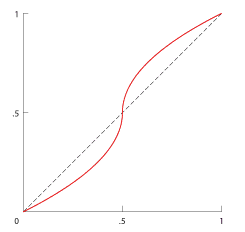
\includegraphics{images/funcion_keener.png}
		\caption{Gráfico de la función $h(x)$.} \label{fig:func_skew}
	\end{figure}

En el caso de que no todos los equipos hubieran jugado el mismo número de partidos habría que normalizar los datos.\\

Teniendo en cuenta todo lo anterior ya podemos crear la matriz A compuesta por los $a_{ij}$.

\subsubsection*{\underline{Planteamiento del problema de autovalores y autovectores}}
\begin{defi} 
	La \textbf{fuerza relativa} de un equipo $i$ comparada con $j$ viene dada por: 
	\begin{equation}
		s_{ij} = a_{ij}r_{j}
	\end{equation}
\end{defi}


\begin{defi} 
	La \textbf{fuerza absoluta} es el resultado de la suma de todas las fuerzas relativas, es decir: 
	\begin{equation}
		s_{i}=\sum_{j=1}^{m} s_{ij} = \sum_{j=1}^{m} a_{ij}r_{j} 
	\end{equation}
	o de forma matricial:
	
	\begin{equation}
		s=
		\begin{array}{ccccccc}
			\left(\begin{array}{c}
				s_{1}\\
				s_{2}\\
				\vdots\\
				s_{m}	
			\end{array}\right) & \begin{array}{c}
			=
		\end{array} & \left(\begin{array}{cccc}
		a_{11} & a_{12} & \dots & a_{1m}\\
		a_{21} & a_{22} & \dots & a_{2m} \\
		\vdots & \vdots & \ddots & \vdots\\
		a_{m1} & a_{m2} & \dots & a_{mm}
	\end{array} \right) & \left(\begin{array}{c}
	r_{1}\\
	r_{2}\\
	\vdots\\
	r_{m}
	\end{array} \right) 
	\end{array}  
	=Ar \label{eqkeener}
	\end{equation}
\end{defi}


	
Según la segunda condición de Keener $s= \lambda r$, a la que aplicando (\ref{eqkeener}) queda de la siguiente forma:
\begin{equation} \label{eqkeener2}
Ar= \lambda r
\end{equation}
En términos de álgebra lineal el vector de ratings $r$ debe ser un autovector y la constante $\lambda$ debe ser el autovalor asociado. Resolver el problema de autovalores y autovectores puede parecer sencillo pero pueden surgir varios problemas:
\begin{itemize}
	\item Para una matriz $m$x$m$ podemos tener $m$ valores distintos para $\lambda$. ¿Cuál elegimos sabiendo que el valor elegido afectará a todo el rating?
	\item Podríamos obtener valores complejos de $\lambda$ que no podríamos comparar.
	\item También podríamos obtener valores negativos tanto de $\lambda$ como del vector $r$.
	\item Calcular los autovalores y autovectores no es un problema sencillo computacionalmente y se necesita software especializado.
\end{itemize}

\subsubsection*{\underline{Restricciones}}
Para superarlos, Keener impone las siguientes tres restricciones:\\
\fbox{\parbox[b]{\linewidth}{
\textbf{I. No negatividad}: cada $a_{ij} \geqslant 0$. \\

\textbf{II. Irreducibilidad}: debe haber suficientes resultados en la competición para asegurar que se pueden comparar dos equipos cualesquiera. Si $i$ y $j$ son dos equipos distintos deben estar conectados por una serie de enfrentamientos que incluye a otros equipos $\{k_{1},k_{2},...,k_{p}\}$ de forma que se tiene una cadena de enfrentamientos\\ 
\begin{equation}
	i \longleftrightarrow k_{1} \longleftrightarrow k_{2} \longleftrightarrow ... \longleftrightarrow k_{p} \longleftrightarrow j \label{eqIrre}
\end{equation}


\textbf{III. Primitiva}: Es una versión más exigente de II en la que requerimos además que cada par de equipos esté conectado por un número uniforme de enfrentamientos. Es decir, para (\ref{eqIrre}) debe existir un único valor $p$ igual para todos los $i$ y $j$.\\
}}
\ \\
Se puede forzar a que la matriz A cumpla II y III haciendo unas pequeñas perturbaciones de la matriz.
\begin{itemize}
	\item Para forzar a que sea irreducible aplicamos lo siguiente:
	\begin{equation*}
	A \leftarrow A + \epsilon e e^{T}
	\end{equation*}
	donde $e$ es una columna de todo 1 y $\epsilon>0$ es un valor relativamente pequeño respecto al valor más pequeño distinto de cero de la matriz original $A$.\\ 
	\item Si la matriz ya es irreducible, para que sea primitiva aplicamos una perturbación similar a la anterior, simulando un enfrentamiento de un equipo consigo mismo, es decir, solo tenemos que perturbar la diagonal principal de $A$.
	\begin{equation*}
	A \leftarrow A + \epsilon e e^{T}
	\end{equation*}
	donde $e^{T} = \left( 0,0,...,0,1,0,...,0 \right) $ y $\epsilon>0$ es un valor relativamente pequeño respecto al valor más pequeño distinto de cero de la matriz original $A$.\\
\end{itemize}

\subsubsection*{\underline{Resolución del problema}}
Imponiendo las restricciones I y II descritas antes podemos usar la teoría de Perron-Frobenius \cite[pág 36]{cap4} \cite{perron} para obtener un vector de ratings de Keener único para la ecuación (\ref{eqkeener2}).\\

Vamos a explicar como se calcularía aplicando el método de la potencia, que se apoya en el hecho de que cuando $k$ aumenta, las potencias $A^{k}$ de $A$ aplicada a cualquier vector positivo $x_{0}$ hace que el producto $A^{k} x_{0}$ tienda hacia el vector $r$.

\begin{equation}
r = \lim\limits_{k \rightarrow \infty}\dfrac{A^{k} x_{0}}{\sum_{i=1}^{m}A^{k} x_{0}} 
\end{equation}
 
El cálculo del vector $r$ por el método de la potencia se realiza de la siguiente manera:\\

Primero seleccionamos un vector $x_{0}$ inicial con el que comenzar el proceso. Por ejemplo:\\
\begin{equation*}
x_{0} = 
\left( \begin{array}{c}
1/m\\
1/m\\
\vdots\\
1/m
\end{array}\right) 
\end{equation*}
 
Y ahora podemos calcular $r$ mediante los siguientes cálculos sucesivos:

\begin{equation}
y_{k}=Ax_{k}, \ \nu_{k}=\sum_{i=1}^{m}(y_{k})_{i}, \ x_{k+1}=\dfrac{y_{k}}{\nu_{k}}, \ para \ k = 0,1,2,... \label{powerm}
\end{equation}
 
De forma que mediante cálculos sucesivos vayamos obteniendo:

\begin{equation*}
x_{1}=\dfrac{Ax_{0}}{\sum_{i=1}^{m}(Ax_{0})_{i}} \ ,
\end{equation*}

\begin{equation*}
x_{2}=\dfrac{Ax_{1}}{\sum_{i=1}^{m}(Ax_{1})_{i}} = \dfrac{A^{2}x_{0}}{\sum_{i=1}^{m}(A^{2}x_{0})_{i}} \ ,
\end{equation*}

\begin{equation*}
x_{3}=\dfrac{Ax_{2}}{\sum_{i=1}^{m}(Ax_{2})_{i}} = \dfrac{A^{3}x_{0}}{\sum_{i=1}^{m}(A^{3}x_{0})_{i}} \ , \ \dots
\end{equation*}

Debemos repetir el proceso sucesivamente obteniendo mayor número de decimales y una mejor aproximación hasta que veamos que los resultados no cambian sustancialmente. La condición de que la matriz es primitiva garantiza que $x_{k} \rightarrow r$ cuando $k \rightarrow \infty$.\\
El esquema del algoritmo puede ser encontrado en \cite{power_method}.

\begin{ejem} Vamos a aplicar el método de Keener a nuestro ejemplo.\\
\end{ejem}
	$\blacksquare $ Vamos a tomar $a_{ij} = \text{nº de partidos que } i \text{ ha ganado a } j $, obteniendo:
	
{\tiny 	\[
	\left(\begin{array}{cccccccccccccccccc}
	0 & 2 & 1 & 1 & 1 & 1 & 0 & 0 & 1 & 0 & 0 & 0 & 2 & 0 & 1 & 0 & 1 & 1\\
	0 & 0 & 2 & 0 & 0 & 2 & 0 & 1 & 2 & 1 & 2 & 1 & 1 & 0 & 1 & 2 & 2 & 2\\
	1 & 0 & 0 & 1 & 1 & 1 & 2 & 1 & 2 & 1 & 2 & 2 & 1 & 1 & 1 & 1 & 0 & 2\\
	1 & 2 & 1 & 0 & 1 & 2 & 1 & 2 & 2 & 1 & 2 & 2 & 1 & 1 & 1 & 2 & 2 & 1\\
	1 & 2 & 1 & 1 & 0 & 2 & 1 & 1 & 2 & 1 & 2 & 0 & 1 & 0 & 1 & 2 & 1 & 0\\
	1 & 0 & 1 & 0 & 0 & 0 & 0 & 1 & 2 & 0 & 1 & 2 & 0 & 0 & 1 & 0 & 0 & 1\\
	2 & 2 & 0 & 1 & 1 & 2 & 0 & 1 & 1 & 1 & 2 & 1 & 1 & 0 & 1 & 1 & 0 & 1\\
	2 & 1 & 1 & 0 & 1 & 1 & 1 & 0 & 1 & 1 & 1 & 1 & 2 & 0 & 1 & 1 & 0 & 0\\
	1 & 0 & 0 & 0 & 0 & 0 & 1 & 1 & 0 & 0 & 1 & 1 & 1 & 1 & 1 & 1 & 1 & 1\\
	2 & 1 & 1 & 1 & 1 & 2 & 1 & 1 & 2 & 0 & 1 & 1 & 1 & 1 & 2 & 0 & 0 & 1\\
	2 & 0 & 0 & 0 & 0 & 1 & 0 & 1 & 1 & 1 & 0 & 1 & 1 & 0 & 0 & 0 & 0 & 0\\
	2 & 1 & 0 & 0 & 2 & 0 & 1 & 1 & 1 & 1 & 1 & 0 & 1 & 0 & 0 & 1 & 0 & 0\\
	0 & 1 & 1 & 1 & 1 & 2 & 1 & 0 & 1 & 1 & 1 & 1 & 0 & 1 & 1 & 1 & 0 & 0\\
	2 & 2 & 1 & 1 & 2 & 2 & 2 & 2 & 1 & 1 & 2 & 2 & 1 & 0 & 2 & 1 & 1 & 2\\
	1 & 1 & 1 & 1 & 1 & 1 & 1 & 1 & 1 & 0 & 2 & 2 & 1 & 0 & 0 & 1 & 1 & 0\\
	2 & 0 & 1 & 0 & 0 & 2 & 1 & 1 & 1 & 2 & 2 & 1 & 1 & 1 & 1 & 0 & 0 & 1\\
	1 & 0 & 2 & 0 & 1 & 2 & 2 & 2 & 1 & 2 & 2 & 2 & 2 & 1 & 1 & 2 & 0 & 2\\
	1 & 0 & 0 & 1 & 2 & 1 & 1 & 2 & 1 & 1 & 2 & 2 & 2 & 0 & 2 & 1 & 0 & 0\\
	\end{array} \right) 
	\]}
	
	
	$\blacksquare $ Todos los $a_{ij} \geqslant 0$.\\
	
	$\blacksquare $ Aplicando (\ref{formejem6}) obtenemos la matriz A:\\
{\tiny 	\[
	\left(\begin{array}{cccccccccccccccccc}
	 1/4 & 3/4 & 1/2 & 1/2 & 1/2 & 1/2 & 1/4 & 1/4 & 1/2 & 1/4 & 1/4 & 1/4 & 3/4 & 1/4 & 1/2 & 1/4 & 1/2 & 1/2 \\
	 1/4 & 1/4 & 3/4 & 1/4 & 1/4 & 3/4 & 1/4 & 1/2 & 3/4 & 1/2 & 3/4 & 1/2 & 1/2 & 1/4 & 1/2 & 3/4 & 3/4 & 3/4 \\
	 1/2 & 1/4 & 1/4 & 1/2 & 1/2 & 1/2 & 3/4 & 1/2 & 3/4 & 1/2 & 3/4 & 3/4 & 1/2 & 1/2 & 1/2 & 1/2 & 1/4 & 3/4 \\
	 1/2 & 3/4 & 1/2 & 1/4 & 1/2 & 3/4 & 1/2 & 3/4 & 3/4 & 1/2 & 3/4 & 3/4 & 1/2 & 1/2 & 1/2 & 3/4 & 3/4 & 1/2 \\
	 1/2 & 3/4 & 1/2 & 1/2 & 1/4 & 3/4 & 1/2 & 1/2 & 3/4 & 1/2 & 3/4 & 1/4 & 1/2 & 1/4 & 1/2 & 3/4 & 1/2 & 1/4 \\
	 1/2 & 1/4 & 1/2 & 1/4 & 1/4 & 1/4 & 1/4 & 1/2 & 3/4 & 1/4 & 1/2 & 3/4 & 1/4 & 1/4 & 1/2 & 1/4 & 1/4 & 1/2 \\
	 3/4 & 3/4 & 1/4 & 1/2 & 1/2 & 3/4 & 1/4 & 1/2 & 1/2 & 1/2 & 3/4 & 1/2 & 1/2 & 1/4 & 1/2 & 1/2 & 1/4 & 1/2 \\
	 3/4 & 1/2 & 1/2 & 1/4 & 1/2 & 1/2 & 1/2 & 1/4 & 1/2 & 1/2 & 1/2 & 1/2 & 3/4 & 1/4 & 1/2 & 1/2 & 1/4 & 1/4 \\
	 1/2 & 1/4 & 1/4 & 1/4 & 1/4 & 1/4 & 1/2 & 1/2 & 1/4 & 1/4 & 1/2 & 1/2 & 1/2 & 1/2 & 1/2 & 1/2 & 1/2 & 1/2 \\
	 3/4 & 1/2 & 1/2 & 1/2 & 1/2 & 3/4 & 1/2 & 1/2 & 3/4 & 1/4 & 1/2 & 1/2 & 1/2 & 1/2 & 3/4 & 1/4 & 1/4 & 1/2 \\
	 3/4 & 1/4 & 1/4 & 1/4 & 1/4 & 1/2 & 1/4 & 1/2 & 1/2 & 1/2 & 1/4 & 1/2 & 1/2 & 1/4 & 1/4 & 1/4 & 1/4 & 1/4 \\
	 3/4 & 1/2 & 1/4 & 1/4 & 3/4 & 1/4 & 1/2 & 1/2 & 1/2 & 1/2 & 1/2 & 1/4 & 1/2 & 1/4 & 1/4 & 1/2 & 1/4 & 1/4 \\
	 1/4 & 1/2 & 1/2 & 1/2 & 1/2 & 3/4 & 1/2 & 1/4 & 1/2 & 1/2 & 1/2 & 1/2 & 1/4 & 1/2 & 1/2 & 1/2 & 1/4 & 1/4 \\
	 3/4 & 3/4 & 1/2 & 1/2 & 3/4 & 3/4 & 3/4 & 3/4 & 1/2 & 1/2 & 3/4 & 3/4 & 1/2 & 1/4 & 3/4 & 1/2 & 1/2 & 3/4 \\
	 1/2 & 1/2 & 1/2 & 1/2 & 1/2 & 1/2 & 1/2 & 1/2 & 1/2 & 1/4 & 3/4 & 3/4 & 1/2 & 1/4 & 1/4 & 1/2 & 1/2 & 1/4 \\
	 3/4 & 1/4 & 1/2 & 1/4 & 1/4 & 3/4 & 1/2 & 1/2 & 1/2 & 3/4 & 3/4 & 1/2 & 1/2 & 1/2 & 1/2 & 1/4 & 1/4 & 1/2 \\
	 1/2 & 1/4 & 3/4 & 1/4 & 1/2 & 3/4 & 3/4 & 3/4 & 1/2 & 3/4 & 3/4 & 3/4 & 3/4 & 1/2 & 1/2 & 3/4 & 1/4 & 3/4 \\
	 1/2 & 1/4 & 1/4 & 1/2 & 3/4 & 1/2 & 1/2 & 3/4 & 1/2 & 1/2 & 3/4 & 3/4 & 3/4 & 1/4 & 3/4 & 1/2 & 1/4 & 1/4 	
	 \end{array} \right) 
	\]}
	
	$\blacksquare $ Como no estamos trabajando con puntuaciones de ningún tipo no hace falta aplicar ninguna función de skewing.\\
	
	$\blacksquare $ Todos los equipos han jugado dos partidos contra cada rival, uno de ida y otro de vuelta, por lo que no hace falta normalizar.\\ 
	
	$\blacksquare $ La matriz es primitiva y, por tanto, irreducible, ya que tenemos resultados para todos los pares de equipos, por lo que no necesitamos aplicar ninguna perturbación.\\
	
	$\blacksquare $ Ya podemos aplicar el método de la potencia.\\
	
	
	Seleccionamos el vector inicial.
	\begin{equation*}
	x_{0} = 
	\left( \begin{array}{c}
	1/18\\
	1/18\\
	1/18\\
	1/18\\
	1/18\\
	1/18\\
	1/18\\
	1/18\\
	1/18\\
	1/18\\
	1/18\\
	1/18\\
	1/18\\
	1/18\\
	1/18\\
	1/18\\
	1/18\\
	1/18
	\end{array}\right) 
	\end{equation*}
	
	\newpage
	
	Ahora seguimos el algoritmo antes explicado en (\ref{powerm}) y vamos obteniendo los siguientes resultados a medida que avanza el proceso:
	
	\begin{equation*}
	\begin{array}{cccc}
	x_{0} = 
	\left( \begin{array}{c}
	0.0556\\
	0.0556\\
	0.0556\\
	0.0556\\
	0.0556\\
	0.0556\\
	0.0556\\
	0.0556\\
	0.0556\\
	0.0556\\
	0.0556\\
	0.0556\\
	0.0556\\
	0.0556\\
	0.0556\\
	0.0556\\
	0.0556\\
	0.0556\\
	\end{array}\right) &
	
	x_{1} = 
	\left( \begin{array}{c}
    0.0476\\
    0.0587\\
    0.0603\\
    0.0683\\
    0.0587\\
    0.0444\\
    0.0571\\
    0.0524\\
    0.0460\\
    0.0587\\
    0.0413\\
    0.0476\\
    0.0508\\
    0.0714\\
    0.0540\\
    0.0556\\
    0.0683\\
    0.0587
	\end{array}\right)
	
	x_{2} = 
	\left( \begin{array}{c}
    0.0490\\
    0.0588\\
    0.0603\\
    0.0685\\
    0.0587\\
    0.0439\\
    0.0565\\
    0.0520\\
    0.0469\\
    0.0587\\
    0.0408\\
    0.0477\\
    0.0516\\
    0.0715\\
    0.0539\\
    0.0550\\
    0.0681\\
    0.0581
	\end{array}\right)	
	
	x_{3} = 
	\left( \begin{array}{c}
    0.0490\\
    0.0587\\
    0.0602\\
    0.0685\\
    0.0587\\
    0.0439\\
    0.0565\\
    0.0521\\
    0.0469\\
    0.0588\\
    0.0409\\
    0.0478\\
    0.0516\\
    0.0715\\
    0.0539\\
    0.0550\\
    0.0680\\
    0.0581
	\end{array}\right)
		
	
	\end{array}
	\end{equation*}
	
	Paramos el refinamiento en $x_{3}$. El valor de $\lambda = 8.5653$
	
	\[r=
	\begin{array}{ccc}
	\left(\begin{array}{c}
    0.0490\\
    0.0587\\
    0.0602\\
    0.0685\\
    0.0587\\
    0.0439\\
    0.0565\\
    0.0521\\
    0.0469\\
    0.0588\\
    0.0409\\
    0.0478\\
    0.0516\\
    0.0715\\
    0.0539\\
    0.0550\\
    0.0680\\
    0.0581
	\end{array} \right) & \left(\begin{array}{c}
    14\\
    6\\
    4\\
    2\\
    7\\
    17\\
    9\\
    12\\
    16\\
    5\\
    18\\
    15\\
    13\\
    1\\
    11\\
    10\\
    3\\
    8
	\end{array} \right) & \begin{array}{c}
	\text{Baloncesto Sevilla}\\
	\text{CAI Zaragoza} \\
	\text{Dominion Bilbao Basket} \\
	\text{FC Barcelona} \\
	\text{FIATC Joventut} \\
	\text{Gipuzkoa Basket} \\
	\text{Herbalife Gran Canaria} \\
	\text{Iberostar Tenerife} \\
	\text{La Bruixa d'Or Manresa} \\
	\text{Laboral Kutxa Baskonia} \\
	\text{Montakit Fuenlabrada} \\
	\text{MoraBanc Andorra} \\
	\text{Movistar Estudiantes} \\
	\text{Real Madrid} \\
	\text{Río Natura Monbús Obradoiro} \\
	\text{UCAM Murcia} \\
	\text{Unicaja Málaga} \\
	\text{Valencia Basket Club}
	\end{array}
	\end{array}
	\]
\qed


\subsection{Método de rating ataque-defensa}
Al que también nos referiremos en adelante como el método ``O-D'' de la traducción del inglés ``Offense-Defense Method''. El objetivo es asignar a cada equipo un rating de ataque $ o_{i} $ y un rating de defensa $d_{i}$ a partir de las estadísticas acumuladas de los partidos. Para aplicarlo vamos a tener en cuenta las puntuaciones a favor y en contra de los enfrentamientos.\\

Un equipo será bueno atacando cuando marque muchos puntos a sus oponentes, en especial a los contrincantes con una buena defensa. Por el contrario, un equipo será bueno defensivamente cuando consiga que sus rivales, en especial los que son buenos en ataque, consigan puntuaciones bajas. Ambos conceptos están fuertemente entrelazados, es decir, existe una función $f$ que relaciona cada rating defensivo con todos los de ataque y una función $g$ que relaciona cada rating de ataque con todos los ratings defensivos.\\

Vamos a construir nuestra matriz de resultados $A$ donde $a_{ij}$ es la puntuación que el equipo $j$ marca a su rival $i$. Esto se puede interpretar como un indicador de ataque para el equipo $j$ y como un indicador de defensa para el equipo $i$. De forma que, si tenemos $m$ equipos, las funciones $f$ y $g$ antes mencionadas que relacionan ambos conceptos quedarían así definidas: 
\begin{itemize}
	\item El rating de ataque del equipo $j$ es:
	\begin{equation}
	o_{j} = \dfrac{a_{1j}}{d_{1}} + \dfrac{a_{2j}}{d_{2}} + \dots + \dfrac{a_{mj}}{d_{m}}  \label{ofens}
	\end{equation} 
	donde $\{d_{1},d_{2}, \dots ,d_{m}\}$ es un conjunto de ratings defensivos. 
	\item El rating de defensa del equipo $i$ es:
	\begin{equation}
	d_{i} = \dfrac{a_{i1}}{o_{1}} + \dfrac{a_{i2}}{o_{2}} + \dots + \dfrac{a_{im}}{o_{m}}  \label{defens}
	\end{equation} 
	donde $\{o_{1},o_{2}, \dots ,o_{m}\}$ es un conjunto de ratings de ataque. 
\end{itemize}

Se tendrá un mejor ataque cuanto mayor sea $o_{j}$ y una mejor defensa cuanto menor sea $d_{i}$.\\
Aplicando las fórmulas anteriores, conseguir muchos puntos frente a equipos con una baja defensa no aumentará de forma considerable el valor total del rating de ataque, pero si lo hace frente a un equipo con una buena defensa, el denominador es relativamente pequeño, lo que incrementará el valor final del rating de ataque. De forme similar ocurre con el rating defensivo, hacer que equipos buenos atacando consigan puntuaciones bajas tendrá mayor valor que contra equipos ofensivamente débiles.\\

Para calcular los ratings $o$ y $d$, debemos comenzar inicializando uno de ellos, por ejemplo, el defensivo con valores positivos arbitrarios:

\[d_{0}=
\left(\begin{array}{c}
1\\
1\\
\vdots \\
1
\end{array} \right)
\]

A partir de $d_{0}$ podemos calcular $o_{1}$ usando (\ref{ofens}). Posteriormente podemos usar los valores obtenidos de $o_{1}$ para calcular valores más exactos de la defensa y hallar $d_{1}$ aplicando (\ref{defens}).\\
Repitiendo sucesivamente este proceso generamos dos secuencias de vectores $\{d_{0},d_{1},\dots\}$ y $\{o_{1},o_{2},\dots\}$. Si las secuencias convergen, tendremos los vectores de ratings de ataque y defensa para los $m$ equipos.
 
\begin{center}
	$
\lim\limits_{k \rightarrow \infty} d_{k} = d = \left(\begin{array}{c}
d_{e1}\\
d_{e2}\\
\vdots \\
d_{em}
\end{array} \right)$      
\ \ \ \ \ \ \ \ \ \ \ \ \
$
\lim\limits_{k \rightarrow \infty} o_{k} = o = \left(\begin{array}{c}
o_{e1}\\
o_{e2}\\
\vdots \\
o_{em}
\end{array} \right)$
\end{center}
 

Matricialmente el problema a resolver queda

\begin{equation}
o_{k} = A^{T} d_{k-1}^{\div} \label{ataq}
\end{equation}
\begin{equation}
d_{k} = A o_{k}^{\div} \label{defen}
\end{equation}
para $k=1,2,3,\dots$ donde
\begin{center}
	\begin{tabular}{ccc}
		\hline  $o_{n\text{x}1}$ & & vector de ratings de ataque a calcular \\
		\hline  $d_{n\text{x}1}$ & & vector de ratings de defensa a calcular \\
		\hline $A_{m\text{x}m}=[a_{ij}]$ & & $a_{ij}=\text{puntuación que marca } j \text{ a } i$  \\ 
		\hline  $o_{n\text{x}1}^{\div}$ & & vector de inversos de $o = 		\left(\begin{array}{c}
		1/o_{e1}\\
		1/o_{e2}\\
		\vdots \\
		1/o_{em}
		\end{array} \right)$ \\
		\hline  $d_{n\text{x}1}^{\div}$ & & vector de inversos de $d = 		\left(\begin{array}{c}
		1/d_{e1}\\
		1/d_{e2}\\
		\vdots \\
		1/d_{em}
		\end{array} \right)$ \\
		\hline 
	\end{tabular}
\end{center} 

empezando con
$d_{0}=
\left(\begin{array}{c}
1\\
1\\
\vdots \\
1
\end{array} \right) $.
\ \\
\ \\
\ \\
\ \\
Una vez hemos obtenido $o$ y $d$ para cada equipo, podemos combinar ambos en un solo rating haciendo para cada $i$
\begin{equation}
r_{i}= \dfrac{o_{i}}{d_{i}} \label{ODr}
\end{equation}
\ \\

Puede ocurrir que $o$ y $d$ no existan porque las secuencias no llegan a converger. En \cite[pág 87-90]{cap7} podemos encontrar un análisis completo del teorema que nos va a decir cuando los vectores van a converger y cuando no basándose en el Teorema de Sinkhor-Knopp.
\begin{teo}
	Las secuencias (\ref{ataq}) y (\ref{defen}) convergen a los vectores $o$ y $d$ respectivamente si y solo si todos los valores positivos de $A$ se encuentran en alguna diagonal positiva, es decir, si A tiene soporte total. 
\end{teo}
Podemos encontrar la demostración en \cite[pág 90-91]{cap7}.\\
    
\begin{ejem} Vamos a aplicar el método de ataque-defensa a nuestro ejemplo.\\
\end{ejem}	
	Construimos la matriz A:
{\tiny 	\[ %esta es la traspuesta
	\left(\begin{array}{cccccccccccccccccc}
	0 & 88 & 70.5 & 84 & 70.5 & 65 & 70.5 & 74 & 75 & 71.5 & 74.5 & 61 & 78 & 76.5 & 81.5 & 75.5 & 75.5 & 76 \\
	85 & 0 & 79 & 67 & 70.5 & 74 & 70.5 & 69.5 & 77.5 & 75 & 77.5 & 71.5 & 71.5 & 72.5 & 75.5 & 78.5 & 86 & 89 \\
	79 & 67.5 & 0 & 73 & 87 & 79.5 & 80 & 84 & 81.5 & 83.5 & 82 & 80 & 70.5 & 70.5 & 71 & 73.5 & 83.5 & 80 \\
	86.5 & 96.5 & 73.5 & 0 & 90.5 & 64 & 75 & 83.5 & 94.5 & 90.5 & 83.5 & 77.5 & 86 & 77 & 73 & 83 & 94 & 74.5 \\
	72.5 & 76 & 88.5 & 72 & 0 & 78.5 & 79 & 85.5 & 83 & 75.5 & 81 & 74 & 70 & 84 & 71.5 & 77 & 79.5 & 78.5 \\
	71.5 & 63 & 73 & 50.5 & 64.5 & 0 & 71 & 72.5 & 80.5 & 64 & 75 & 77.5 & 75 & 73 & 83 & 67.5 & 65.5 & 77.5 \\
	77 & 93.5 & 67 & 68.5 & 79 & 72.5 & 0 & 73.5 & 78 & 81.5 & 82 & 88 & 77 & 68.5 & 70 & 84.5 & 67.5 & 91 \\
	89 & 74.5 & 84.5 & 72.5 & 87 & 76.5 & 67.5 & 0 & 69.5 & 82.5 & 82.5 & 70.5 & 80 & 83.5 & 79.5 & 79.5 & 69.5 & 77 \\
	76 & 67 & 76.5 & 61 & 71 & 69.5 & 77 & 68.5 & 0 & 65.5 & 66 & 76 & 77 & 78 & 71 & 76 & 72.5 & 79.5 \\
	95.5 & 83.5 & 80.5 & 84 & 84.5 & 87 & 93 & 70 & 79 & 0 & 80 & 87 & 85 & 84 & 83 & 82.5 & 76.5 & 82 \\
	76.5 & 68 & 69.5 & 73 & 69 & 75.5 & 71 & 78.5 & 71.5 & 81 & 0 & 86.5 & 86 & 81.5 & 72.5 & 67.5 & 69 & 70 \\
	83 & 75.5 & 73.5 & 65 & 83 & 70.5 & 86 & 64.5 & 80 & 80.5 & 73 & 0 & 68 & 76.5 & 69 & 72.5 & 71.5 & 77.5 \\
	65 & 72 & 73 & 82 & 69 & 86.5 & 73.5 & 70 & 76.5 & 72.5 & 85 & 67 & 0 & 77.5 & 69 & 77.5 & 70 & 71.5 \\
	84 & 84.5 & 78.5 & 79.5 & 85.5 & 88 & 79 & 93.5 & 81.5 & 78 & 91 & 81.5 & 88 & 0 & 88 & 84.5 & 92 & 94.5 \\
	74 & 75.5 & 67.5 & 68 & 72.5 & 89.5 & 68.5 & 58 & 73.5 & 75.5 & 81.5 & 76 & 58.5 & 74.5 & 0 & 84 & 73.5 & 65 \\
	97 & 67 & 82.5 & 67 & 62 & 84.5 & 88.5 & 88 & 75.5 & 89 & 76.5 & 73.5 & 79 & 75.5 & 60 & 0 & 71 & 74 \\
	76 & 81 & 90 & 85.5 & 77.5 & 75 & 75.5 & 86.5 & 78.5 & 82 & 75 & 80 & 75.5 & 88 & 73 & 88 & 0 & 82 \\
	84 & 91.5 & 76.5 & 75 & 89 & 88 & 87.5 & 89.5 & 80.5 & 86.5 & 88 & 80 & 82.5 & 79 & 77 & 78.5 & 74.5 & 0 	
	\end{array} \right) 
	\]}
	
	Seleccionamos el vector inicial:
	\begin{equation*}
		d_{0} = 
		\left( \begin{array}{c}
			1\\
			1\\
			\vdots\\
			1
		\end{array}\right) 
	\end{equation*}
	Aplicando (\ref{ataq}) y (\ref{defen}), los vectores $o$ y $d$ no tardan en converger y aplicando solo 3 iteraciones del proceso hallamos los valores para los ratings:
	
	\[o=
	\begin{array}{ccc}
	\left(\begin{array}{c}
				1271.9\\
				1289.8\\
				1325.5\\
				1397.6\\
				1325.9\\
				1204.3\\
				1318\\
				1324.9\\
				1228.8\\
				1418.9\\
				1269.1\\
				1268.2\\
				1257.8\\
				1453\\
				1232.4\\
				1309.9\\
				1368.7\\
				1409.1
	\end{array} \right) & \left(\begin{array}{c}
				12\\
				11\\
				7\\
				4\\
				6\\
				18\\
				9\\
				8\\
				17\\
				2\\
				13\\
				14\\
				15\\
				1\\
				16\\
				10\\
				5\\
				3
	\end{array} \right) & \begin{array}{c}
	\text{Baloncesto Sevilla}\\
	\text{CAI Zaragoza} \\
	\text{Dominion Bilbao Basket} \\
	\text{FC Barcelona} \\
	\text{FIATC Joventut} \\
	\text{Gipuzkoa Basket} \\
	\text{Herbalife Gran Canaria} \\
	\text{Iberostar Tenerife} \\
	\text{La Bruixa d'Or Manresa} \\
	\text{Laboral Kutxa Baskonia} \\
	\text{Montakit Fuenlabrada} \\
	\text{MoraBanc Andorra} \\
	\text{Movistar Estudiantes} \\
	\text{Real Madrid} \\
	\text{Río Natura Monbús Obradoiro} \\
	\text{UCAM Murcia} \\
	\text{Unicaja Málaga} \\
	\text{Valencia Basket Club}
	\end{array}
	\end{array}
	\]
	
	
	\[d=
	\begin{array}{ccc}
	\left(\begin{array}{c}
	1.0406\\
	1.0044\\
	0.9928\\
	0.9355\\
	0.9964\\
	1.0029\\
	0.9988\\
	0.9944\\
	1.0130\\
	1.0187\\
	1.0278\\
	0.9930\\
	0.9914\\
	1.0109\\
	0.9614\\
	1.0116\\
	0.9837\\
	1.0229
	\end{array} \right) & \left(\begin{array}{c}
	18\\
	11\\
	5\\
	1\\
	8\\
	10\\
	9\\
	7\\
	14\\
	15\\
	17\\
	6\\
	4\\
	12\\
	2\\
	13\\
	3\\
	16
	\end{array} \right) & \begin{array}{c}
	\text{Baloncesto Sevilla}\\
	\text{CAI Zaragoza} \\
	\text{Dominion Bilbao Basket} \\
	\text{FC Barcelona} \\
	\text{FIATC Joventut} \\
	\text{Gipuzkoa Basket} \\
	\text{Herbalife Gran Canaria} \\
	\text{Iberostar Tenerife} \\
	\text{La Bruixa d'Or Manresa} \\
	\text{Laboral Kutxa Baskonia} \\
	\text{Montakit Fuenlabrada} \\
	\text{MoraBanc Andorra} \\
	\text{Movistar Estudiantes} \\
	\text{Real Madrid} \\
	\text{Río Natura Monbús Obradoiro} \\
	\text{UCAM Murcia} \\
	\text{Unicaja Málaga} \\
	\text{Valencia Basket Club}
	\end{array}
	\end{array}
	\]
	
	Combinando ambos en un único ranking usando (\ref{ODr})
	
		\[r=
		\begin{array}{ccc}
		\left(\begin{array}{c}
		    1222.3\\
		    1284.1\\
		    1335.1\\
		    1494\\
		    1330.7\\
		    1200.8\\
		    1319.6\\
		    1332.4\\
		    1213\\
		    1392.9\\
		    1234.8\\
		    1277.1\\
		    1268.7\\
		    1437.3\\
		    1281.9\\
		    1294.9\\
		    1391.4\\
		    1377.6
		\end{array} \right) & \left(\begin{array}{c}
		    16\\
		    11\\
		    6\\
		    1\\
		    8\\
		    18\\
		    9\\
		    7\\
		    17\\
		    3\\
		    15\\
		    13\\
		    14\\
		    2\\
		    12\\
		    10\\
		    4\\
		    5
		\end{array} \right) & \begin{array}{c}
		\text{Baloncesto Sevilla}\\
		\text{CAI Zaragoza} \\
		\text{Dominion Bilbao Basket} \\
		\text{FC Barcelona} \\
		\text{FIATC Joventut} \\
		\text{Gipuzkoa Basket} \\
		\text{Herbalife Gran Canaria} \\
		\text{Iberostar Tenerife} \\
		\text{La Bruixa d'Or Manresa} \\
		\text{Laboral Kutxa Baskonia} \\
		\text{Montakit Fuenlabrada} \\
		\text{MoraBanc Andorra} \\
		\text{Movistar Estudiantes} \\
		\text{Real Madrid} \\
		\text{Río Natura Monbús Obradoiro} \\
		\text{UCAM Murcia} \\
		\text{Unicaja Málaga} \\
		\text{Valencia Basket Club}
		\end{array}
		\end{array}
		\]
\qed
  \ \\ \ \\ \ \\ \ \\ \ \\ 
A modo de resumen y de cara a las siguientes secciones vamos a mostrar todos los rankings que hemos obtenido aplicando los cuatro métodos explicados, respectivamente, Massey, Colley, Keener y el de ataque-defensa:

\begin{equation*} 
\begin{array}{ccccc}
\left(\begin{array}{c}
	16\\
	11\\
	6\\
	1\\
	8\\
	18\\
	9\\
	7\\
	17\\
	3\\
	15\\
	11\\
	14\\
	2\\
	13\\
	10\\
	5\\
	4
\end{array} \right)  & \left(\begin{array}{c}
	14\\
	8\\
	4\\
	2\\
	6\\
	17\\
	8\\
	11\\
	16\\
	6\\
	18\\
	14\\
	13\\
	1\\
	12\\
	10\\
	2\\
	4
\end{array} \right) & \left(\begin{array}{c}
14\\
6\\
4\\
2\\
7\\
17\\
9\\
12\\
16\\
5\\
18\\
15\\
13\\
1\\
11\\
10\\
3\\
8
\end{array} \right) & \left(\begin{array}{c}
16\\
11\\
6\\
1\\
8\\
18\\
9\\
7\\
17\\
3\\
15\\
13\\
14\\
2\\
12\\
10\\
4\\
5
\end{array} \right) & \begin{array}{c}
\text{Baloncesto Sevilla}\\
\text{CAI Zaragoza} \\
\text{Dominion Bilbao Basket} \\
\text{FC Barcelona} \\
\text{FIATC Joventut} \\
\text{Gipuzkoa Basket} \\
\text{Herbalife Gran Canaria} \\
\text{Iberostar Tenerife} \\
\text{La Bruixa d'Or Manresa} \\
\text{Laboral Kutxa Baskonia} \\
\text{Montakit Fuenlabrada} \\
\text{MoraBanc Andorra} \\
\text{Movistar Estudiantes} \\
\text{Real Madrid} \\
\text{Río Natura Monbús Obradoiro} \\
\text{UCAM Murcia} \\
\text{Unicaja Málaga} \\
\text{Valencia Basket Club}
\end{array} 
\end{array} 
\end{equation*}

\section{Agregación de rankings}
En la sección 2.2.4. vimos cómo combinar dos ratings distintos, el de ataque $o$ y el de defensa $d$ mediante (\ref{ODr}) para obtener $r$. Es un ejemplo sencillo de agregación de rankings.\\

En este capítulo usaremos distintos rankings creados aplicando los métodos explicados en la sección anterior para crear una única lista más robusta \cite{cap13-14}. La calidad del ranking obtenido dependerá de lo buenos que sean los rankings usados. 

\subsection{Ranking promedio}

Este método consiste en calcular la media de las posiciones que ocupa cada elemento en los distintos rankings y ordenar el rating ascendentemente. Acepta rankings de entrada que contengan empates y es común que también se produzcan empates en el ranking de salida.\\

\newpage

\begin{ejem} Usando todos los rankings obtenidos aplicando los cuatro métodos explicados en la sección anterior para nuestro ejemplo vamos a calcular el ranking agregado mediante este método.
\end{ejem}
	
	\[
	\begin{array}{ccc}
	\left(\begin{array}{c}
	15\\
	9\\
	5\\
	1.5\\
	7.25\\
	17.5\\
	8.75\\
	9.25\\
	16.5\\
	4.25\\
	16.5\\
	13.25\\
	13.5\\
	1.5\\
	12\\
	10\\
	3.5\\
	5.25
	\end{array} \right) & \left(\begin{array}{c}
	15\\
	9\\
	5\\
	1\\
	7\\
	18\\
	8\\
	10\\
	16\\
	4\\
	16\\
	13\\
	14\\
	1\\
	12\\
	11\\
	3\\
	6
	\end{array} \right) & \begin{array}{c}
	\text{Baloncesto Sevilla}\\
	\text{CAI Zaragoza} \\
	\text{Dominion Bilbao Basket} \\
	\text{FC Barcelona} \\
	\text{FIATC Joventut} \\
	\text{Gipuzkoa Basket} \\
	\text{Herbalife Gran Canaria} \\
	\text{Iberostar Tenerife} \\
	\text{La Bruixa d'Or Manresa} \\
	\text{Laboral Kutxa Baskonia} \\
	\text{Montakit Fuenlabrada} \\
	\text{MoraBanc Andorra} \\
	\text{Movistar Estudiantes} \\
	\text{Real Madrid} \\
	\text{Río Natura Monbús Obradoiro} \\
	\text{UCAM Murcia} \\
	\text{Unicaja Málaga} \\
	\text{Valencia Basket Club}
	\end{array} 
	\end{array} 
	\]	
\qed

\subsection{Suma de Borda}
Data de 1770 cuando Jean-Charles de Borda lo planteó como método para agregar rankings de candidatos tras unas elecciones.\\

Por cada ranking, cada elemento recibe una puntuación igual al número de elementos que supera. Las puntuaciones de cada ranking que vamos a agregar se suman para cada elemento del conjunto y así obtener un número natural que denominaremos suma de Borda. Los rankings de entrada pueden contener empates.\\

A partir del rating obtenido, ordenando descendentemente, obtendremos el ranking agregado. Sin embargo se trata de un método fácilmente manipulable. Podemos ver un ejemplo en \cite[pág 854]{refborda}.

\newpage

\begin{ejem} Usando todos los rankings obtenidos en la sección anterior vamos a calcular el ranking agregado usando la suma de Borda.
\end{ejem}

\begin{center}
	\begin{tabular}{|c||c|c|c|c||c|}
	\hline \rule[-2ex]{0pt}{5.5ex} Equipo & Massey & Colley & Keener & O-D & Suma Borda \\ 
	\hline \rule[-2ex]{0pt}{5.5ex} Baloncesto Sevilla & 2 & 3 & 4 & 2 & 11 \\ 
	\hline \rule[-2ex]{0pt}{5.5ex} CAI Zaragoza & 6 & 9 & 12 & 7 & 34 \\ 
	\hline \rule[-2ex]{0pt}{5.5ex} Dominion Bilbao Basket & 12 & 13 & 14 & 12 & 51 \\ 
	\hline \rule[-2ex]{0pt}{5.5ex} FC Barcelona & 17 & 15 & 16 & 17 & 65 \\ 
	\hline \rule[-2ex]{0pt}{5.5ex} FIATC Joventut & 10 & 11 & 11 & 10 & 42 \\ 
	\hline \rule[-2ex]{0pt}{5.5ex} Gipuzkoa Basket & 0 & 1 & 1 & 0 & 2 \\ 
	\hline \rule[-2ex]{0pt}{5.5ex} Herbalife Gran Canaria & 9 & 9 & 9 & 9 & 36 \\ 
	\hline \rule[-2ex]{0pt}{5.5ex} Iberostar Tenerife & 11 & 7 & 6 & 11 & 35 \\ 
	\hline \rule[-2ex]{0pt}{5.5ex} La Bruixa d'Or Manresa & 1 & 2 & 2 & 1 & 6 \\ 
	\hline \rule[-2ex]{0pt}{5.5ex} Laboral Kutxa Baskonia & 15 & 11 & 13 & 15 & 54 \\ 
	\hline \rule[-2ex]{0pt}{5.5ex} Montakit Fuenlabrada & 3 & 0 & 0 & 3 & 6 \\ 
	\hline \rule[-2ex]{0pt}{5.5ex} MoraBanc Andorra & 6 & 3 & 3 & 5 & 17 \\ 
	\hline \rule[-2ex]{0pt}{5.5ex} Movistar Estudiantes & 4 & 5 & 5 & 4 & 18 \\ 
	\hline \rule[-2ex]{0pt}{5.5ex} Real Madrid & 16 & 17 & 17 & 16 & 66 \\ 
	\hline \rule[-2ex]{0pt}{5.5ex} Río Natura Monbús Obradoiro & 5 & 6 & 7 & 6 & 24 \\ 
	\hline \rule[-2ex]{0pt}{5.5ex} UCAM Murcia & 8 & 8 & 8 & 8 & 32 \\ 
	\hline \rule[-2ex]{0pt}{5.5ex} Unicaja Málaga & 13 & 15 & 15 & 14 & 57 \\ 
	\hline \rule[-2ex]{0pt}{5.5ex} Valencia Basket Club & 14 & 13 & 10 & 13 & 50 \\ 
	\hline 
\end{tabular}
\end{center} 

\newpage

Y ordenando obtenemos el ranking agregado:\\
\[
\begin{array}{cc}
\left(\begin{array}{c}
15\\
10\\
5\\
2\\
7\\
18\\
8\\
9\\
16\\
4\\
16\\
14\\
13\\
1\\
12\\
11\\
3\\
6
\end{array} \right) & \begin{array}{c}
\text{Baloncesto Sevilla}\\
\text{CAI Zaragoza} \\
\text{Dominion Bilbao Basket} \\
\text{FC Barcelona} \\
\text{FIATC Joventut} \\
\text{Gipuzkoa Basket} \\
\text{Herbalife Gran Canaria} \\
\text{Iberostar Tenerife} \\
\text{La Bruixa d'Or Manresa} \\
\text{Laboral Kutxa Baskonia} \\
\text{Montakit Fuenlabrada} \\
\text{MoraBanc Andorra} \\
\text{Movistar Estudiantes} \\
\text{Real Madrid} \\
\text{Río Natura Monbús Obradoiro} \\
\text{UCAM Murcia} \\
\text{Unicaja Málaga} \\
\text{Valencia Basket Club}
\end{array} 
\end{array} 
\]
\qed


\subsection{Método óptimo de agregación de rankings}
Los dos métodos antes vistos son métodos heurísticos, lo que no garantiza que la agregación de rankings sea óptima (aunque sí más rápidos de calcular). El método de agregación de rankings que vamos a explicar a continuación fue propuesto por el Doctor Yoshitsugu Yamamoto y optimiza la conformidad o concordancia entre los rankings de entrada.\\

Si tenemos $n$ ítems en $k$ rankings definimos la matriz $C_{n \text{x} n}$, que representará las concordancias entre los distintos rankings, de la siguiente manera:
\begin{center}
	$c_{ij} = \text{ nº de rankings con }i \text{ por encima de } j \text{ } -  \text{ nº de rankings con }j \text{ por encima de } i \text{ }$,
\end{center}

de forma que $C$ puede estar formada a partir de rankings con empates o de rankings parciales\footnote{Son aquellos rankings que no contienen todos los elementos a ordenar.}.\\

Nuestro objetivo es crear un ranking que maximice las concordancias entre los rankings. 
Para resolver el problema de optimización necesitaremos variables de decisión que formarán la matriz $X_{n \text{x} n}$ y tomarán los siguientes valores
\begin{center}
	$ x_{ij} =  \begin{cases}
1 & \text{ si el ítem \textit{i} debe aparecer por encima del \textit{j} en el ranking} \\
0 & \text{ en otro caso } 
\end{cases}$
\end{center}
Por lo cual, las variables de decisión deben ser binarias, es decir, solo pueden tomar los valores 0 y 1.\\

El equipo $i$ y $j$ deben aparecer en el ranking de una de las siguientes alternativas: $i$ aparece encima de $j$ o $j$ aparece encima de $i$, pero no se puede dar ningún otro caso. Esta restricción del problema es la restricción antisimétrica y la formulamos como $x_{ij} + x_{ji} = 1$ para cada par de ítems $i$ y $j$.\\

Otra cosa a tener en cuenta es la transitividad. Si $i$ aparece encima de $j$ y $j$ se sitúa encima de $k$, entonces $k$ no puede estar por encima de $i$, tiene que aparecer necesariamente por debajo. Esta restricción la formulamos como la inecuación $x_{ij} + x_{jk} + x_{ki} \leq 2$.\\


Por tanto, nuestro problema de optimización BILP\footnote{Binary Integer Linear Program.} a resolver es el siguiente:\\

\begin{equation} \label{optprob}
	max \sum_{i=1}^{n} \sum_{j=1}^{n} c_{ij} x_{ij} \ \ \ \ \ \ \ \ \ \ x_{ij} \in \{0,1\} 
\end{equation}
\begin{equation*}
	x_{ij} + x_{ji} = 1 \ \ \ \ \ \ \ \ \forall (i,j)
\end{equation*}
\begin{equation*}
	x_{ij} + x_{jk} + x_{ki} \leq 2 \ \ \ \forall (i,j,k)
\end{equation*}
con $n(n-1)$ variables de decisión, $n(n-1)$ restricciones antisimétricas y con $n(n-1)(n-2)$ restricciones transitivas. Este $O(n^{3})$ de las restricciones transitivas limitan mucho el tamaño de los problemas a resolver\footnote{donde el tamaño viene dado por el número de ítems de los rankings.}, por lo que se deben buscar estrategias de relajación de restricciones (que trataremos al fin de la sección).\\

Una vez resuelto el problema tendremos la matriz $X$ con 0s y 1s, donde cada 1 representa que el item $i$ debe aparecer por encima del elemento $j$, por tanto, el elemento con mayor número de 1s debe de ser el primero en el ranking. Es decir, para ordenar los elementos basta con obtener la suma de cada fila y ordenarlos ascendentemente.\\   
 
\begin{ejem} En este ejemplo no vamos a aplicar el método para ordenar todos los 18 equipos participantes porque complicaría bastante la formulación y realización del problema de optimización. Por ello se han elegido 5 equipos al azar que son: Iberostar Tenerife, Montakit Fuenlabrada, Real Madrid, Río Natura Monbús Obradoiro y UCAM Murcia.
\end{ejem}	
Construimos la matriz $C$:

\[	
	\left( \begin{array}{ccccc}
		0 & 4 & -4 & 2 & 0\\
		-4 & 0 & -4 & -4 & -4\\
		4 & 4 & 0 & 4 & 4\\
		-2 & 4 & -4 & 0 & -4\\
		0 & 4 & -4 & 4 & 0
	\end{array} \right) 
\]	
\ \\  \ \\
Añadiendo todas las restricciones antisimétricas y transitivas que se necesitan, ya podemos resolver el problema de optimización (\ref{optprob}) .\\

El valor de la función objetivo a maximizar es 34 y la matriz $X$ obtenida es la siguiente: 	
	
\[	
	\left( \begin{array}{ccccc}
	0 & 1 & 0 & 1 & 0\\
	0 & 0 & 0 & 0 & 0\\
	1 & 1 & 0 & 1 & 1\\
	0 & 1 & 0 & 0 & 0\\
	1 & 1 & 0 & 1 & 0
	\end{array} \right) 
\]
	
Ordenando la suma de las filas de la matriz $X$ obtenemos el ranking:

\[
\begin{array}{cc}
\left(\begin{array}{c}
3\\
5\\
1\\
4\\
2
\end{array} \right) & \begin{array}{c}
\text{Iberostar Tenerife} \\
\text{Montakit Fuenlabrada} \\
\text{Real Madrid} \\
\text{Río Natura Monbús Obradoiro} \\
\text{UCAM Murcia} \\
\end{array} 
\end{array} 
\]	
	
\qed	

La solución óptima podría no ser única. Para averiguar si existen varias soluciones óptimas basta con coger cada par de elementos consecutivos en el ranking y ver si pueden ser intercambiados sin que cambie el valor de la función objetivo ni se viole ningunas de las restricciones. En caso positivo, existe otro ranking alternativo que también es óptimo en el que se intercambian de posición los dos elementos en cuestión. En el caso de nuestro ejemplo, esto no ocurre. El ranking óptimo obtenido es único.\\ 

La optimización discreta es más costosa que la optimización continua. Para resolver BILP grandes (con bastantes ítems a ordenar) es conveniente resolverlos como un problema de programación lineal relajado. Básicamente consiste en hacer que las variables $x_{ij}$ que obligábamos a ser binarias y discretas ahora las permitamos ser continuas. El problema a resolver es el siguiente:
\begin{equation} \label{optprob2}
	max \sum_{i=1}^{n} \sum_{j=1}^{n} c_{ij} x_{ij}
\end{equation}
\begin{equation*}
	x_{ij} + x_{ji} = 1 \ \ \ \ \ \ \ \ \forall (i,j)
\end{equation*}
\begin{equation*}
	x_{ij} + x_{jk} + x_{ki} \leq 2 \ \ \ \forall (i,j,k)
\end{equation*}
\begin{equation*}
	x_{ij} \geq 0
\end{equation*}
Cuando la solución solo tiene valores binarios, la solución del problema LP\footnote{Linear Program.} relajado es también óptima para el BILP. Sin embargo, pueden aparecer unos pocos valores fraccionales que representarán la existencia de más de una solución óptima pudiendo intercambiar los equipos en cuestión. En \cite{refbilp} podemos encontrar en detalle las condiciones para identificar cuando la solución de un LP también es óptima para el BILP.\\
En nuestro ejemplo, resolviendo el problema como un LP relajado obtenemos una solución únicamente con valores binarios que coincide con la obtenida resolviendo el BILP. \\

Otra forma de reducir el coste computacional es mediante la relajación de las restricciones transitivas que limitan el tamaño de los problemas (tanto del BILP como del LP relajado) con su complejidad $O(n^{3})$. \\
Este método consiste en inicialmente suponer que todas las restricciones transitivas son innecesarias y resolver el problema sin ellas, cuando obtenemos la solución tenemos que detectar las restricciones de este tipo que son incumplidas y añadirlas a las restricciones que debe cumplir el problema. Debemos repetir este proceso sucesivamente hasta encontrar todas las restricciones transitivas que son necesarias y llegar a la solución óptima del problema.\\


\section{Comparación de rankings}
Una vez que hemos visto varios métodos para crear rankings y formas para agregarlos creando super-rankings es natural que nos preguntemos: ¿Cuál de todos los rankings que tenemos es mejor? Vamos a ver dos formas distintas de comparar rankings. En el fondo el problema reside en estudiar la desviación entre dos rankings \cite{cap16}.

\subsection{Tau de Kendall}
Propuesta por el estadístico Maurice Kendall, se aplica a rankings completos que tienen el mismo número de elementos. \\

\begin{defi} Diremos que un par $(i,j)$ es \textbf{concordante} si la posición relativa entre ambos en las dos listas es la misma, es decir, $i$ aparece por encima de $j$ o $j$ aparece por encima de $i$ en ambos rankings.
\end{defi}

El resultado, que oscila entre -1 y 1, nos da el grado en que un ranking coincide con el otro y lo podemos calcular como se muestra a continuación

\begin{equation}
\tau = \dfrac{n_{c} - n_{d}}{n(n-1)/2}
\end{equation}
donde $n_{c}$ es el número de pares concordantes, $n_{d}$ el de pares discordantes y $n$ número de ítems de los rankings. 

\newpage

\begin{ejem} Vamos a proceder a comparar los rankings obtenidos mediante los métodos de Massey\footnote{En el ranking de Massey se produce un empate en el puesto 11º entre dos equipos. Como de los dos enfrentamientos, cada equipo ganó uno, hemos procedido a desempatar en favor del equipo que sumó más puntos entre los dos encuentros.} ($r_{m}$), Keener ($r_{k}$) y OD ($r_{OD}$) (aparecen todos al final de la sección 2.2).
\end{ejem}
\begin{center}
$ \tau (r_{m},r_{k}) = \dfrac{131-22}{153} = 0.7124$\\
$ \tau (r_{m},r_{OD}) = \dfrac{150-3}{153} = 0.9607$\\
$ \tau (r_{k},r_{OD}) = \dfrac{134-19}{153} = 0.7516$
\end{center}
	
El ranking obtenido por Massey y el obtenido por el método de OD son los más similares, habiendo solo 3 pares de equipos intercambiados entre ellos.

\qed

Existe una adaptación de la Tau de Kendall para rankings parciales y rankings con distintos tamaños que se puede encontrar en \cite[pág 205,206]{cap16}.


\subsection{Rho de Spearman}
La Rho de Spearman es simplemente la distancia $L_{1}$ entre dos rankings completos $r_{1}$ y $r_{2}$ de tamaño $n$:
\begin{equation} \label{Spearman}
	\rho = ||r_{1} - r_{2}||_{1}= \sum_{i=1}^{n} |r_{1}(i) - r_{2}(i)|
\end{equation}
donde $r_{1}(i)$ es el puesto del equipo $i$ en el ranking $r_{1}$ y $r_{2}(i)$ es el puesto del equipo $i$ en el ranking $r_{2}$. \\

Cuanto menor es el valor de esta medida, es porque la diferencia de puestos en los rankings entre los equipos  es menor y, por tanto, más similares son los rankings.
\begin{ejem} Vamos a proceder a comparar los rankings obtenidos mediante los métodos de Massey ($r_{m}$), Keener ($r_{k}$) y OD ($r_{OD}$) (podemos encontrar todos al final de la sección 2.2).
\end{ejem}
	\begin{center}
		$ \rho (r_{m},r_{k}) = 38$\\
		$ \rho (r_{m},r_{OD}) = 6$\\
		$ \rho (r_{k},r_{OD}) = 32$
	\end{center}
	
	El ranking obtenido por Massey y el obtenido por el método de OD son los más similares.
	
\qed

Sin embargo, no es igual de importante la coincidencia de los rankings en las últimas posiciones de la lista como lo es en las primeras. Esto con la Tau de Kendall no podíamos materializarlo, pero podemos redefinir la fórmula de Spearman (\ref{Spearman}) como 
\begin{equation}
	\phi = \sum_{i=1}^{n} \dfrac{|r_{1}(i) - r_{2}(i)|}{min\{r_{1}(i),r_{2}(i)\}}
\end{equation}
de forma que la penalización por las discordancias en los primeros puestos del ranking será mayor que en los puestos bajos de la lista. 

\begin{ejem} Calculamos los valores usando la nueva definición.
\end{ejem}	
	\begin{center}
		$ \phi (r_{m},r_{k}) = 7,777$\\
		$ \phi (r_{m},r_{OD}) = 0,856$\\
		$ \phi (r_{k},r_{OD}) = 6,576$ 
	\end{center}
	
	El ranking obtenido por Massey y el obtenido por el método de OD vuelven a ser los más similares.
	
\qed
\ \\
Podemos hacer una adaptación de la Rho de Spearman para rankings parciales que se puede encontrar en \cite[pág 207-211]{cap16}.

\section{Competitividad en Rankings}
En esta sección vamos ha hacer un estudio de cómo los ítems van intercambiando sus posiciones a lo largo de una secuencia de rankings \cite{refcomp}.\\

\begin{defi} Si tenemos un conjunto $R=\{r_{1},r_{2},\dots,r_{n}\}$ de rankings diremos que el par de ítems $(i,j)$ \textbf{compite} si existen $r_{t} \in \{r_{1},r_{2},\dots,r_{n}\}$ y su consecutivo $r_{t+1}$ de forma que $i$ y $j$ intercambian su posición relativa entre $r_{t}$ y $r_{t+1}$.
\end{defi}

\begin{ejem} A continuación se muestra la posición de los equipos al acabar la primera y la segunda jornada respectivamente.
\end{ejem}
\[
\begin{array}{ccc} 
\begin{array}{c}
\text{Baloncesto Sevilla}\\
\text{CAI Zaragoza} \\
\text{Dominion Bilbao Basket} \\
\text{FC Barcelona} \\
\text{FIATC Joventut} \\
\text{Gipuzkoa Basket} \\
\text{Herbalife Gran Canaria} \\
\text{Iberostar Tenerife} \\
\text{La Bruixa d'Or Manresa} \\
\text{Laboral Kutxa Baskonia} \\
\text{Montakit Fuenlabrada} \\
\text{MoraBanc Andorra} \\
\text{Movistar Estudiantes} \\
\text{Real Madrid} \\
\text{Río Natura Monbús Obradoiro} \\
\text{UCAM Murcia} \\
\text{Unicaja Málaga} \\
\text{Valencia Basket Club}
\end{array} & \left(\begin{array}{c}
11\\
10\\
3\\
2\\
9\\
15\\
13\\
7\\
18\\
17\\
16\\
14\\
4\\
6\\
1\\
8\\
5\\
12
\end{array} \right) & \left(\begin{array}{c}
17\\
12\\
4\\
1\\
6\\
15\\
11\\
10\\
18\\
16\\
14\\
13\\
8\\
2\\
9\\
5\\
3\\
7
\end{array} \right)
\end{array} 
\]  

Los pares (Moviestar Estudiantes, Real Madrid), (Río Natura, FC Barcelona) o (Baloncesto Sevilla, MoraBanc Andorra) compiten ya que la posición relativa de los equipos de un ranking al siguiente cambia.\\

Sin embargo (CAI Zaragoza, UCAM Murcia), (Unicaja Málaga, Montakit Fuenlabrada) o (FC Barcelona, Real Madrid) no compiten porque no intercambian su posición en los rankings.

\qed

\begin{defi} El \textbf{grafo de competitividad} de un conjunto de rankings $R$ se define como un grafo no dirigido $G_{c}(R)=(V,E_{R})$ donde el conjunto de arcos $E_{R}$ viene dado por la regla: existe un arco entre los nodos i y j si (i,j) compite.
\end{defi}

\begin{ejem} En la figura \ref{fig:gcomp} se muestra como queda el grafo de competitividad tras analizar los rankings de las 34 jornadas disputadas de la ACB del año 2014/2015.
\end{ejem}	
	\begin{figure}[H]
		\centering
		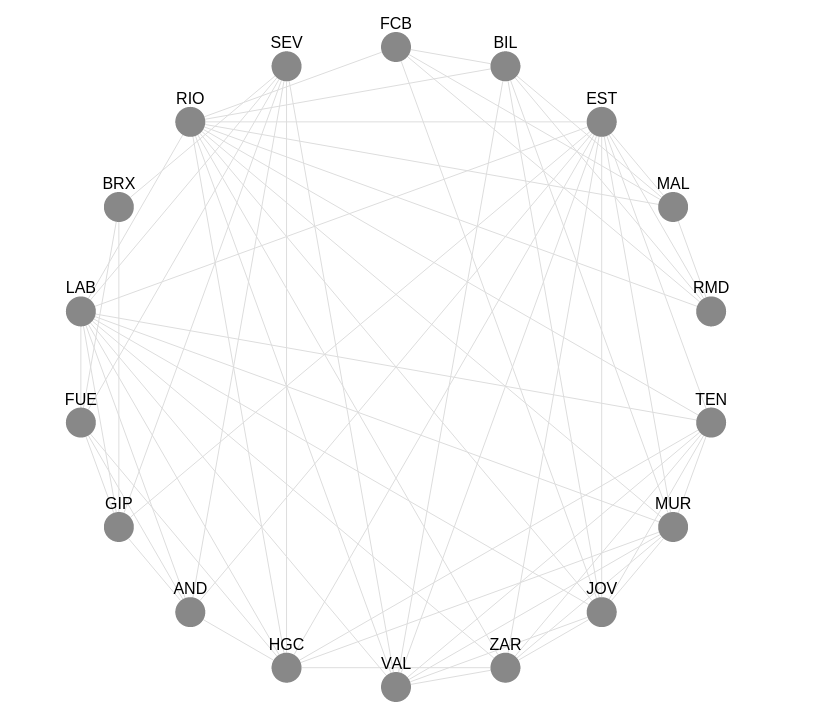
\includegraphics[scale=0.6]{images/Grafo_competitividad.png}
		\caption{Grafo de Competitividad.} \label{fig:gcomp}
	\end{figure}
	
\qed

\ \\

El coste computacional para construir el grafo de competitividad de un conjunto $R$ de $n$ rankings distintos donde los rankings constan de $m$ elementos cada uno es $nm^{2}$.